
\chapter{Performance}


{\centering
\emph{All of the following charts have been included for instructional purposes only.\\Please refer to POH for all calculations of performance.}
\par }

There are two types of charts available for the Duchess that many students are unfamiliar with. A description of these two follows. The rest of the charts are standard.

\section{Accelerate-Stop Distance Defined}

Accelerate-stop distance is the distance required to accelerate to decision speed (71 KIAS for the Duchess) and
brake to a complete stop in the event an engine failure occurs at decision speed. It’s important to realize that
accelerate-stop speed is determined by factory test pilots with prior knowledge of where the failure is to occur.
Therefore, the distances given in the performance charts should be considered the absolute best-case scenario.

\section{Accelerate-Go Distance Defined}

Accelerate-go distance is the distance required to accelerate to decision speed (71 KIAS for the Duchess) and to
continue the takeoff and clear a 50 FT obstacle in the event an engine failure occurs at decision speed. An
accelerate-go distance is only applicable if the airplane can get airborne under the prevailing conditions (weight,
density altitude); single-engine climb performance may not be possible with the gear down.

As with accelerate-stop distance, accelerate-go distance figures are determined by factory test pilots with prior
knowledge of where the failure is to occur. Regard the distances given in the performance charts as the absolute
best-case scenario.

\emph{Memory aid: Any weight 3,600 lbs or more is \underline{always} a no-go!
Do an \underline{accelerate-stop} instead.}

\section{Takeoff Distance}

\begin{figure}[H]
\begin{center}
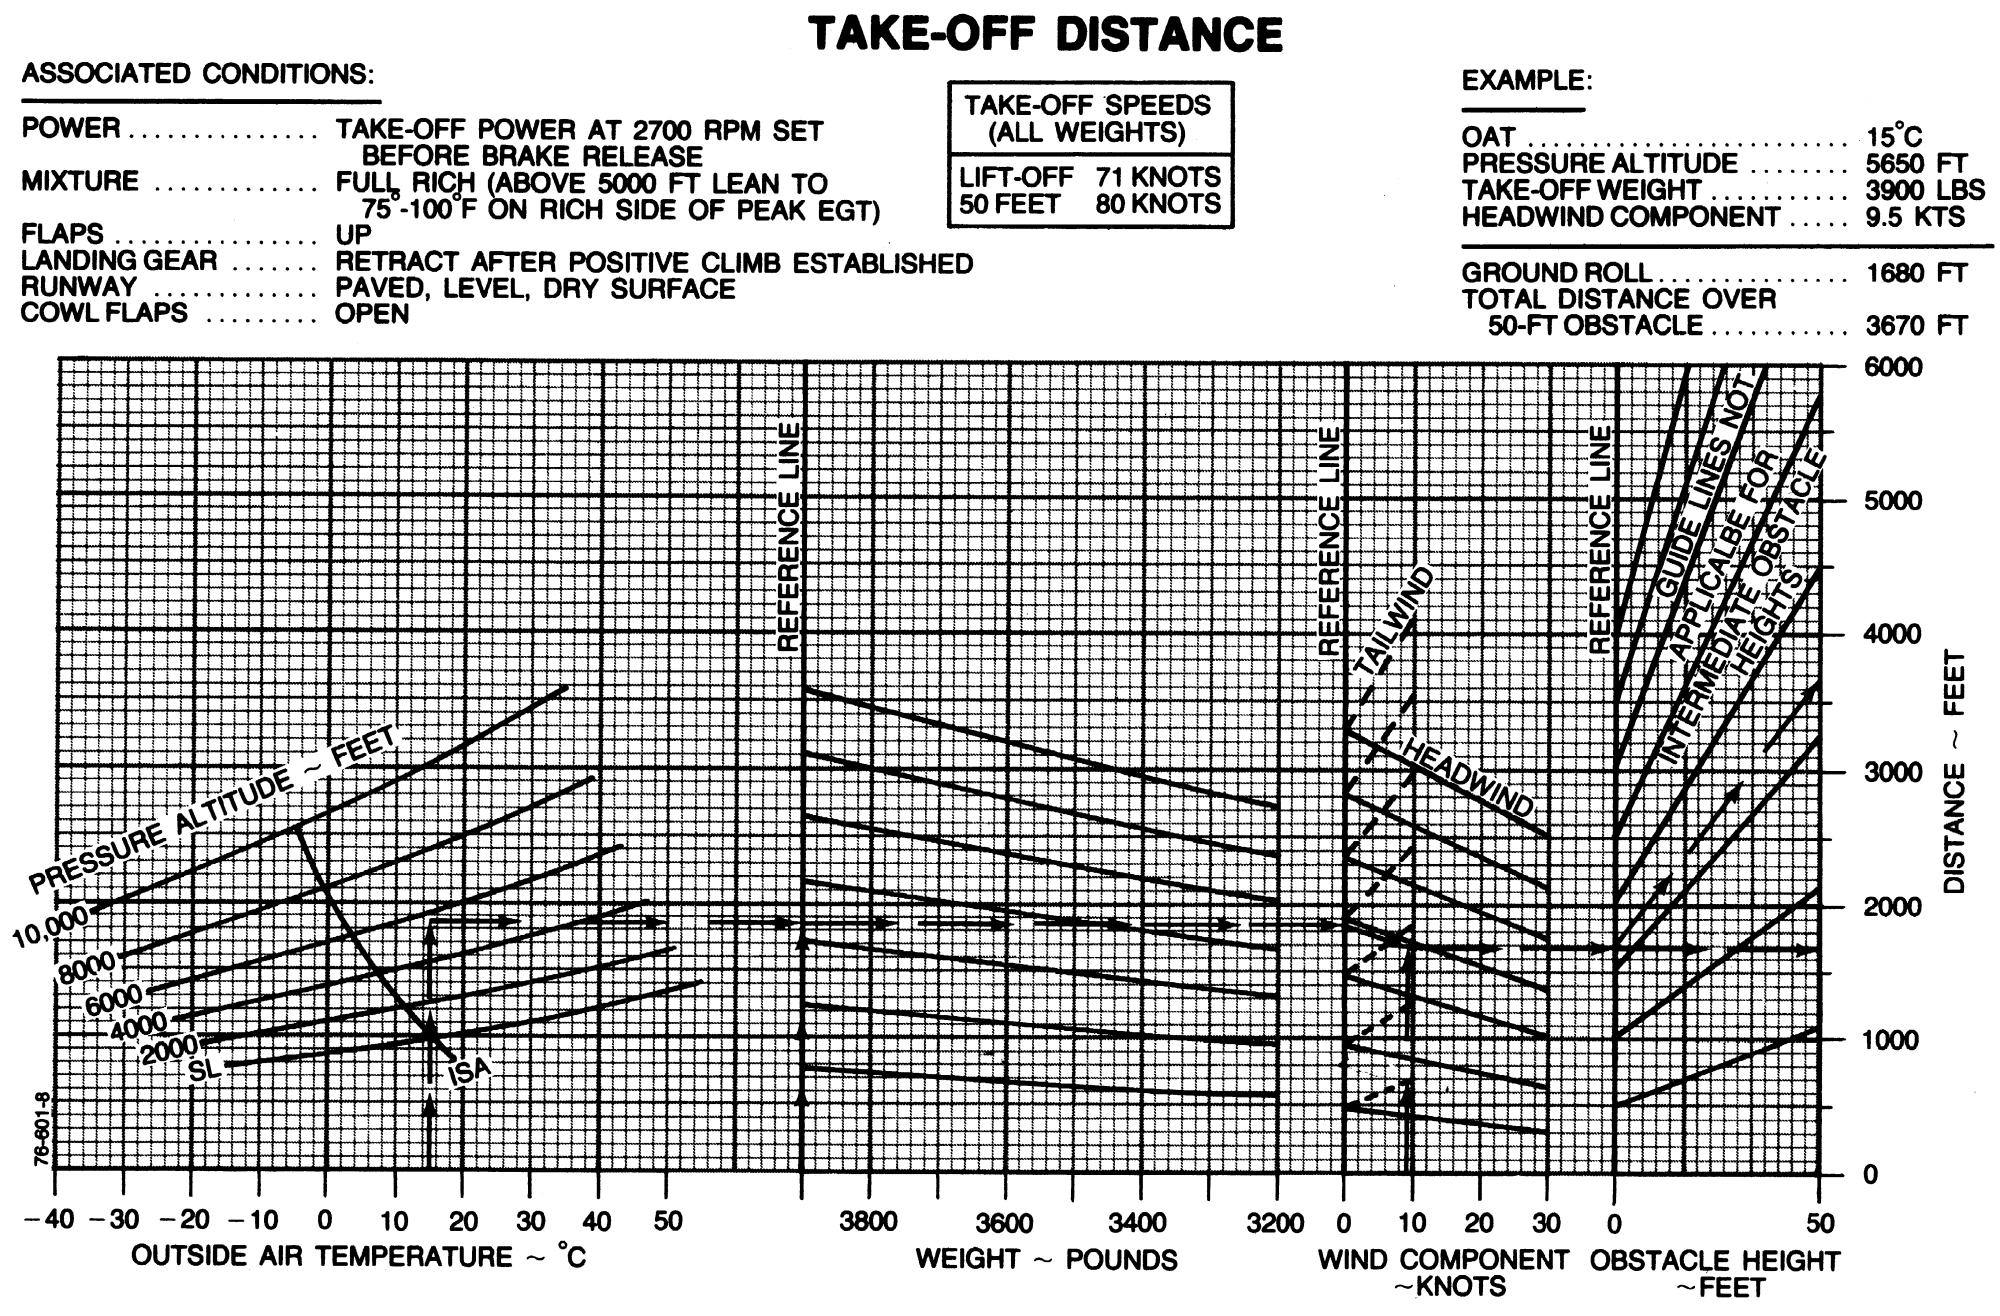
\includegraphics[width=0.95\linewidth]{duchess-takeoff-distance}
\end{center}
\end{figure}

\section{Accelerate-Stop Distance}

\begin{figure}[H]
\begin{center}
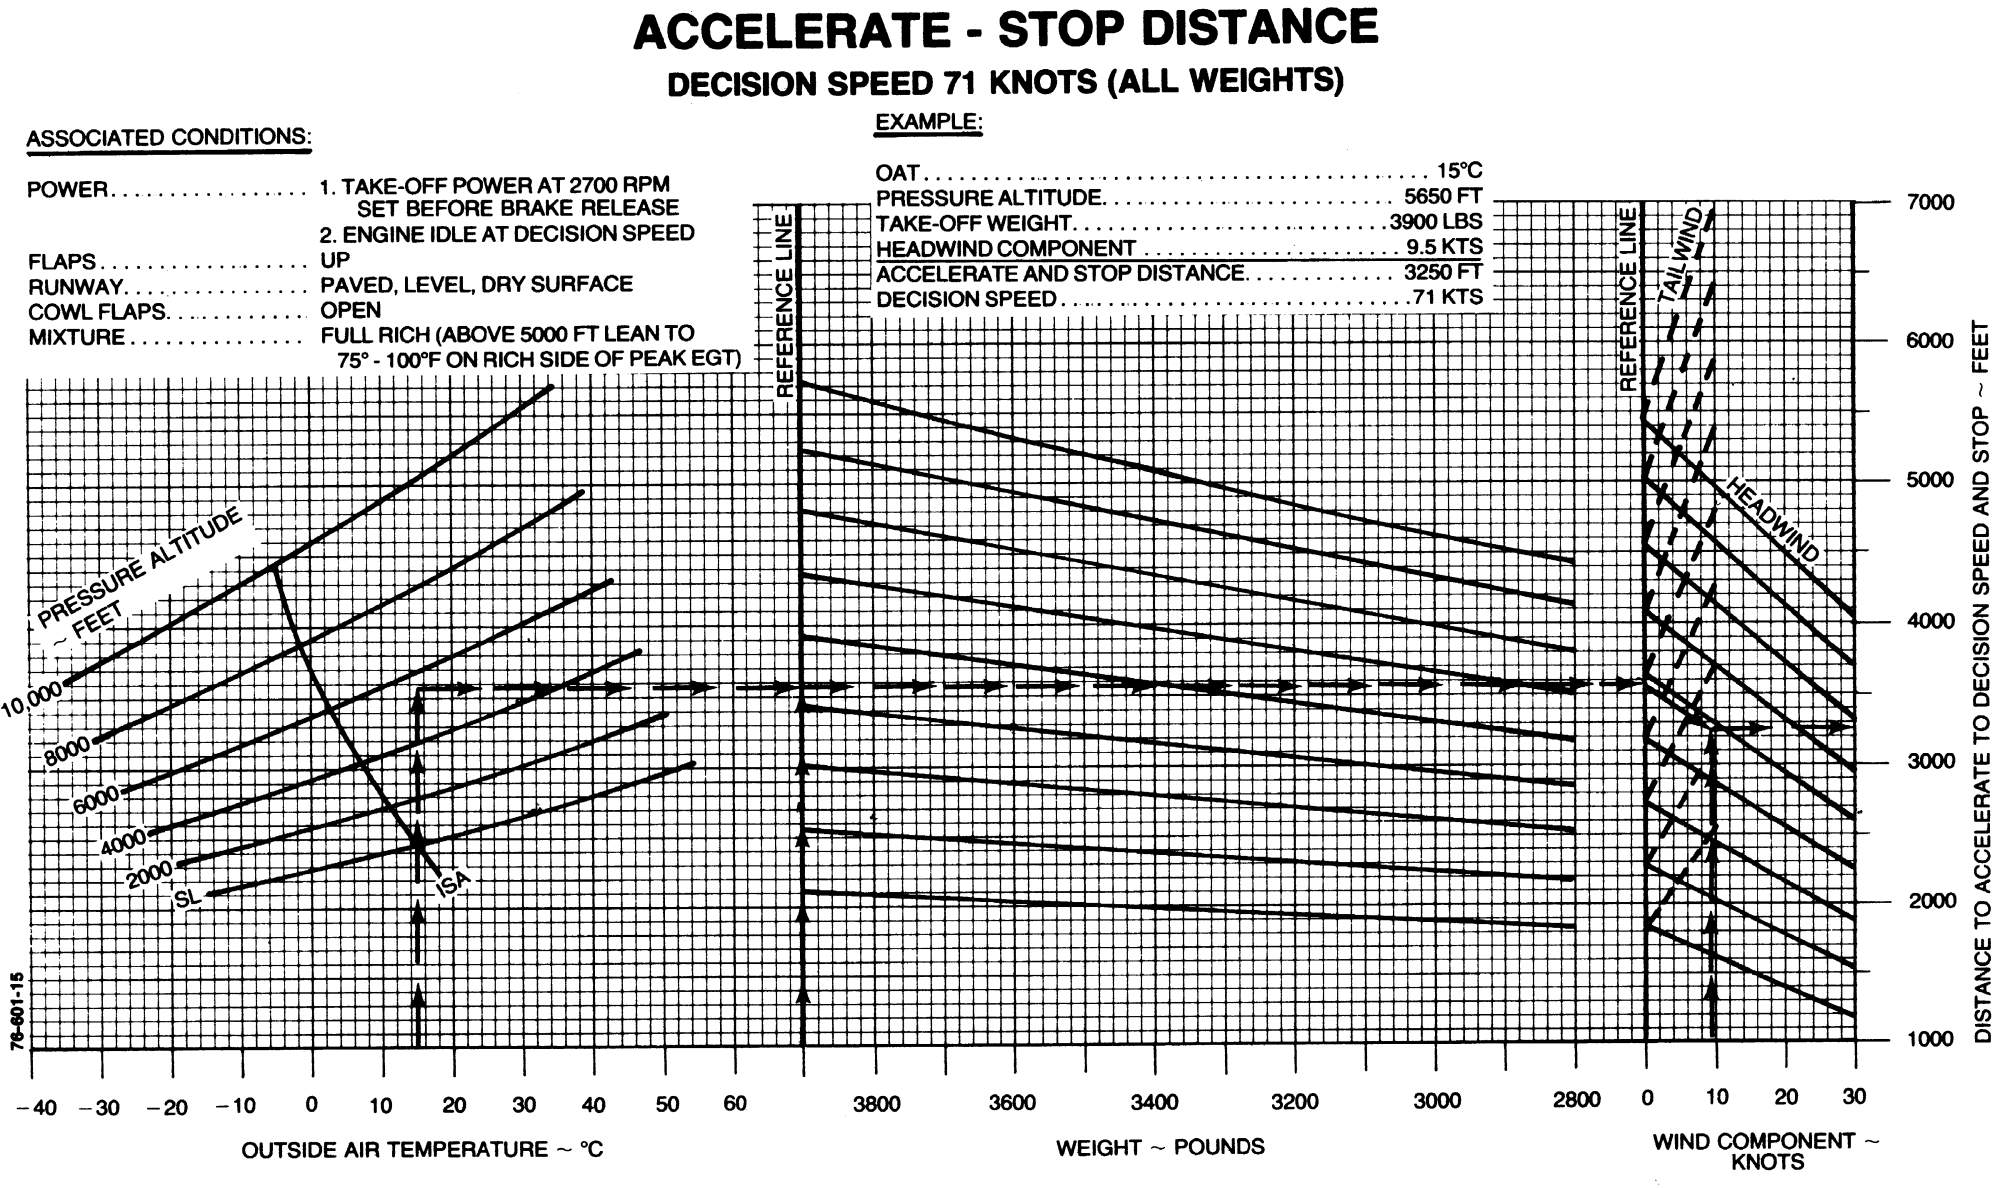
\includegraphics[width=0.95\linewidth]{duchess-asda}
\end{center}
\end{figure}

\section{Accelerate-Go Distance}

\begin{figure}[H]
\begin{center}
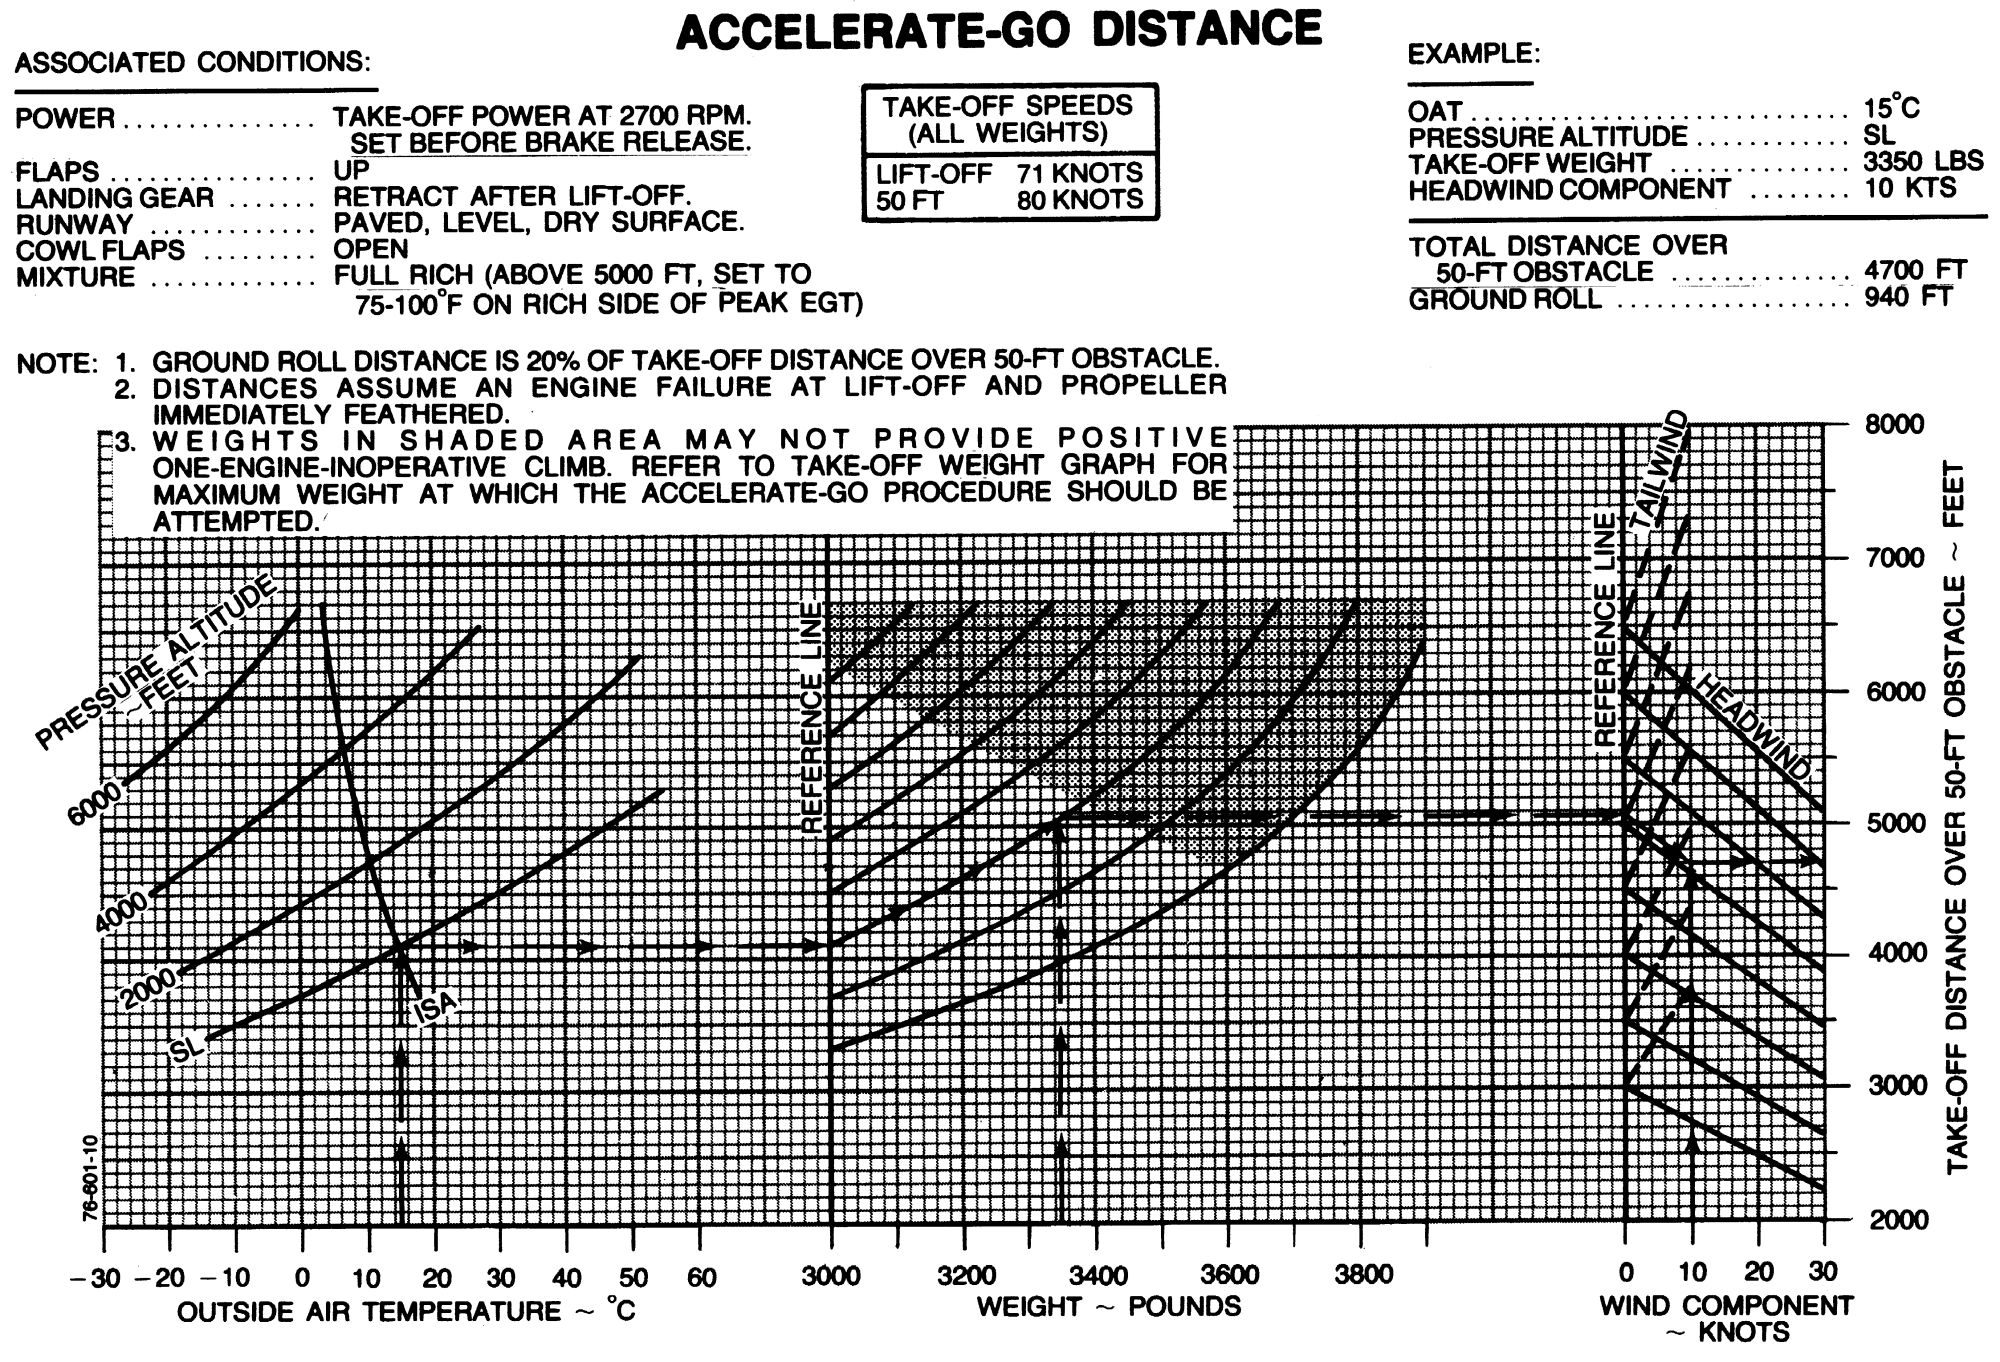
\includegraphics[width=0.95\linewidth]{duchess-accel-go}
\end{center}
\end{figure}

\newpage

\section{Two-Engine Climb Rate}

\begin{figure}[H]
\begin{center}
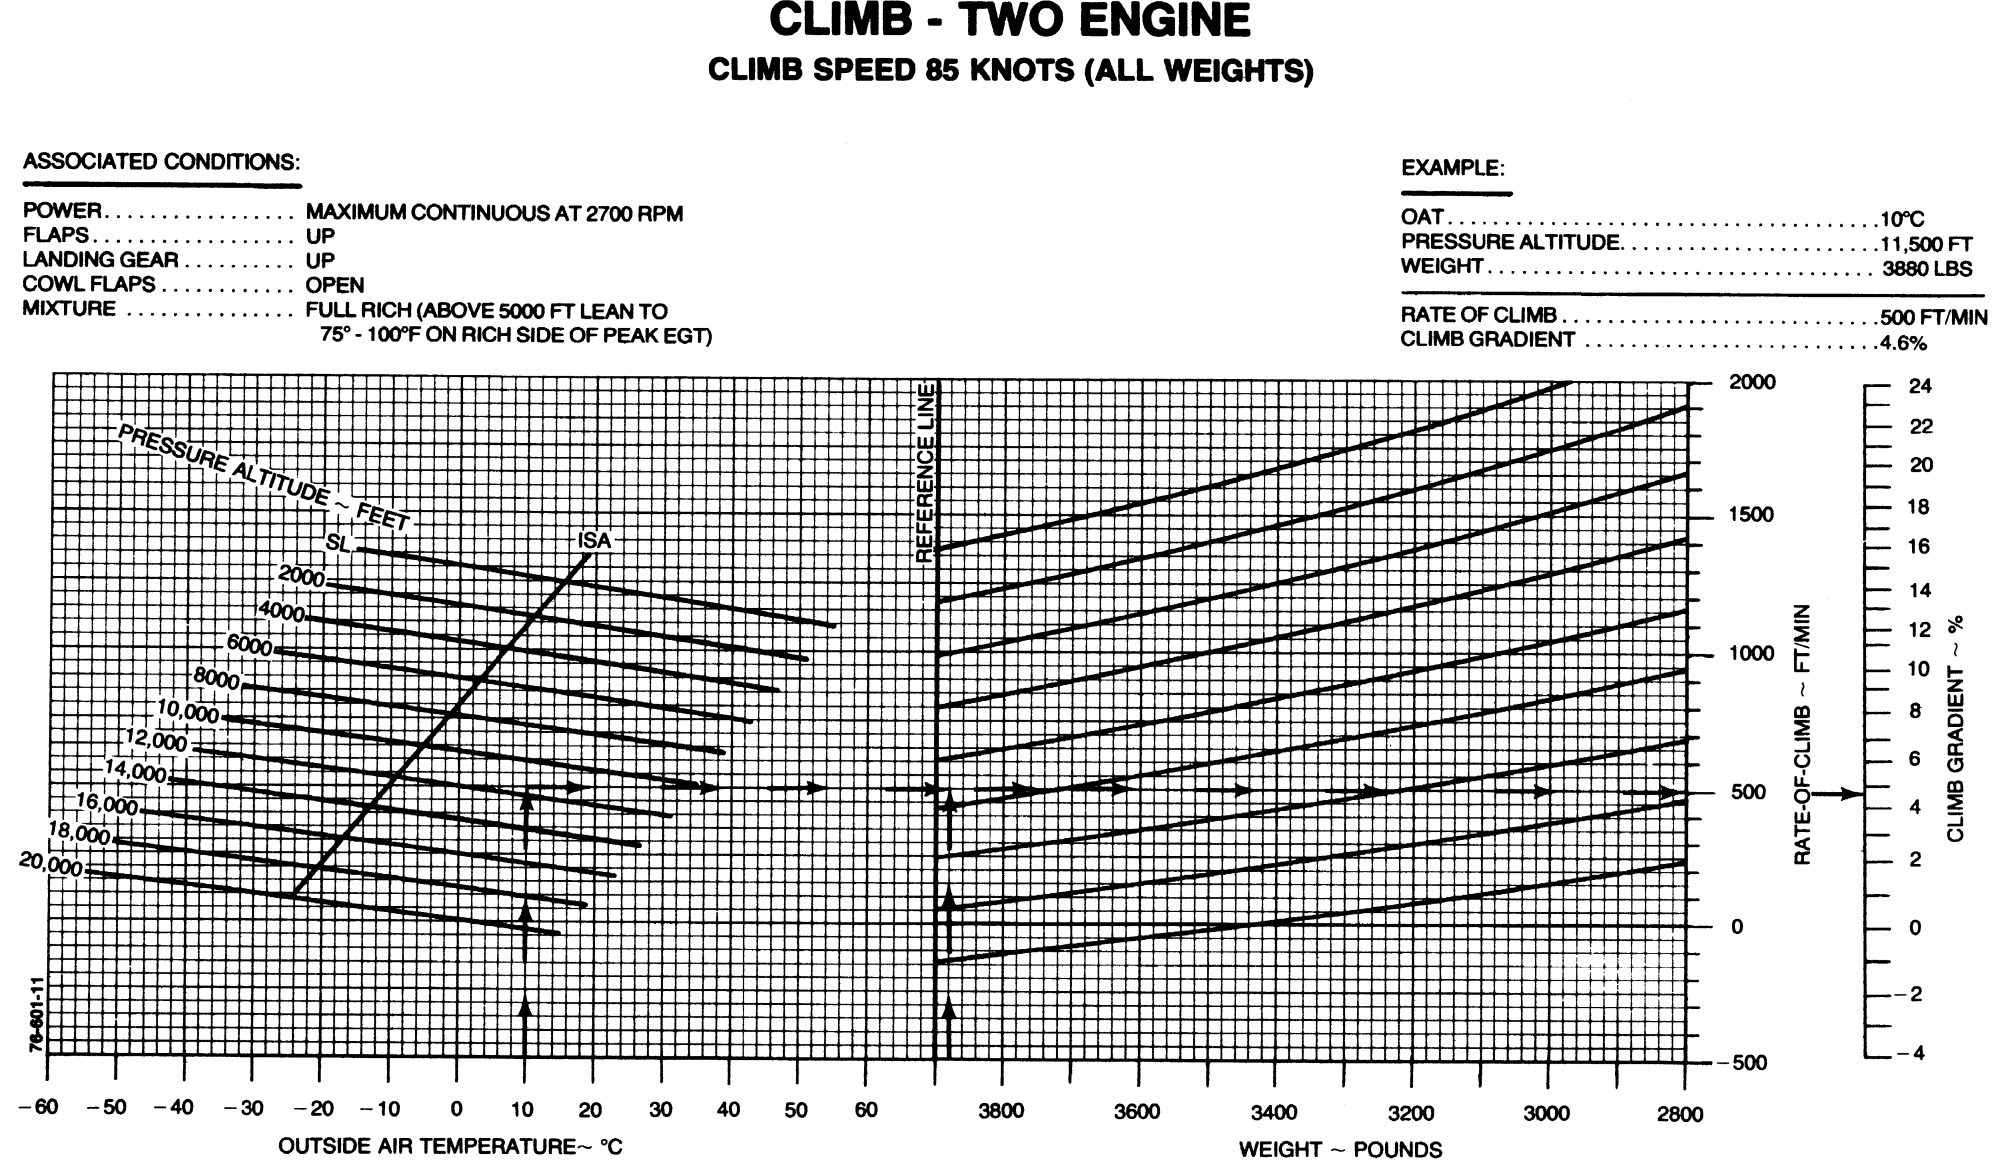
\includegraphics[width=0.9\linewidth]{duchess-2ec}
\end{center}
\end{figure}


\section{Single-Engine Climb Rate}

\begin{figure}[H]
\begin{center}
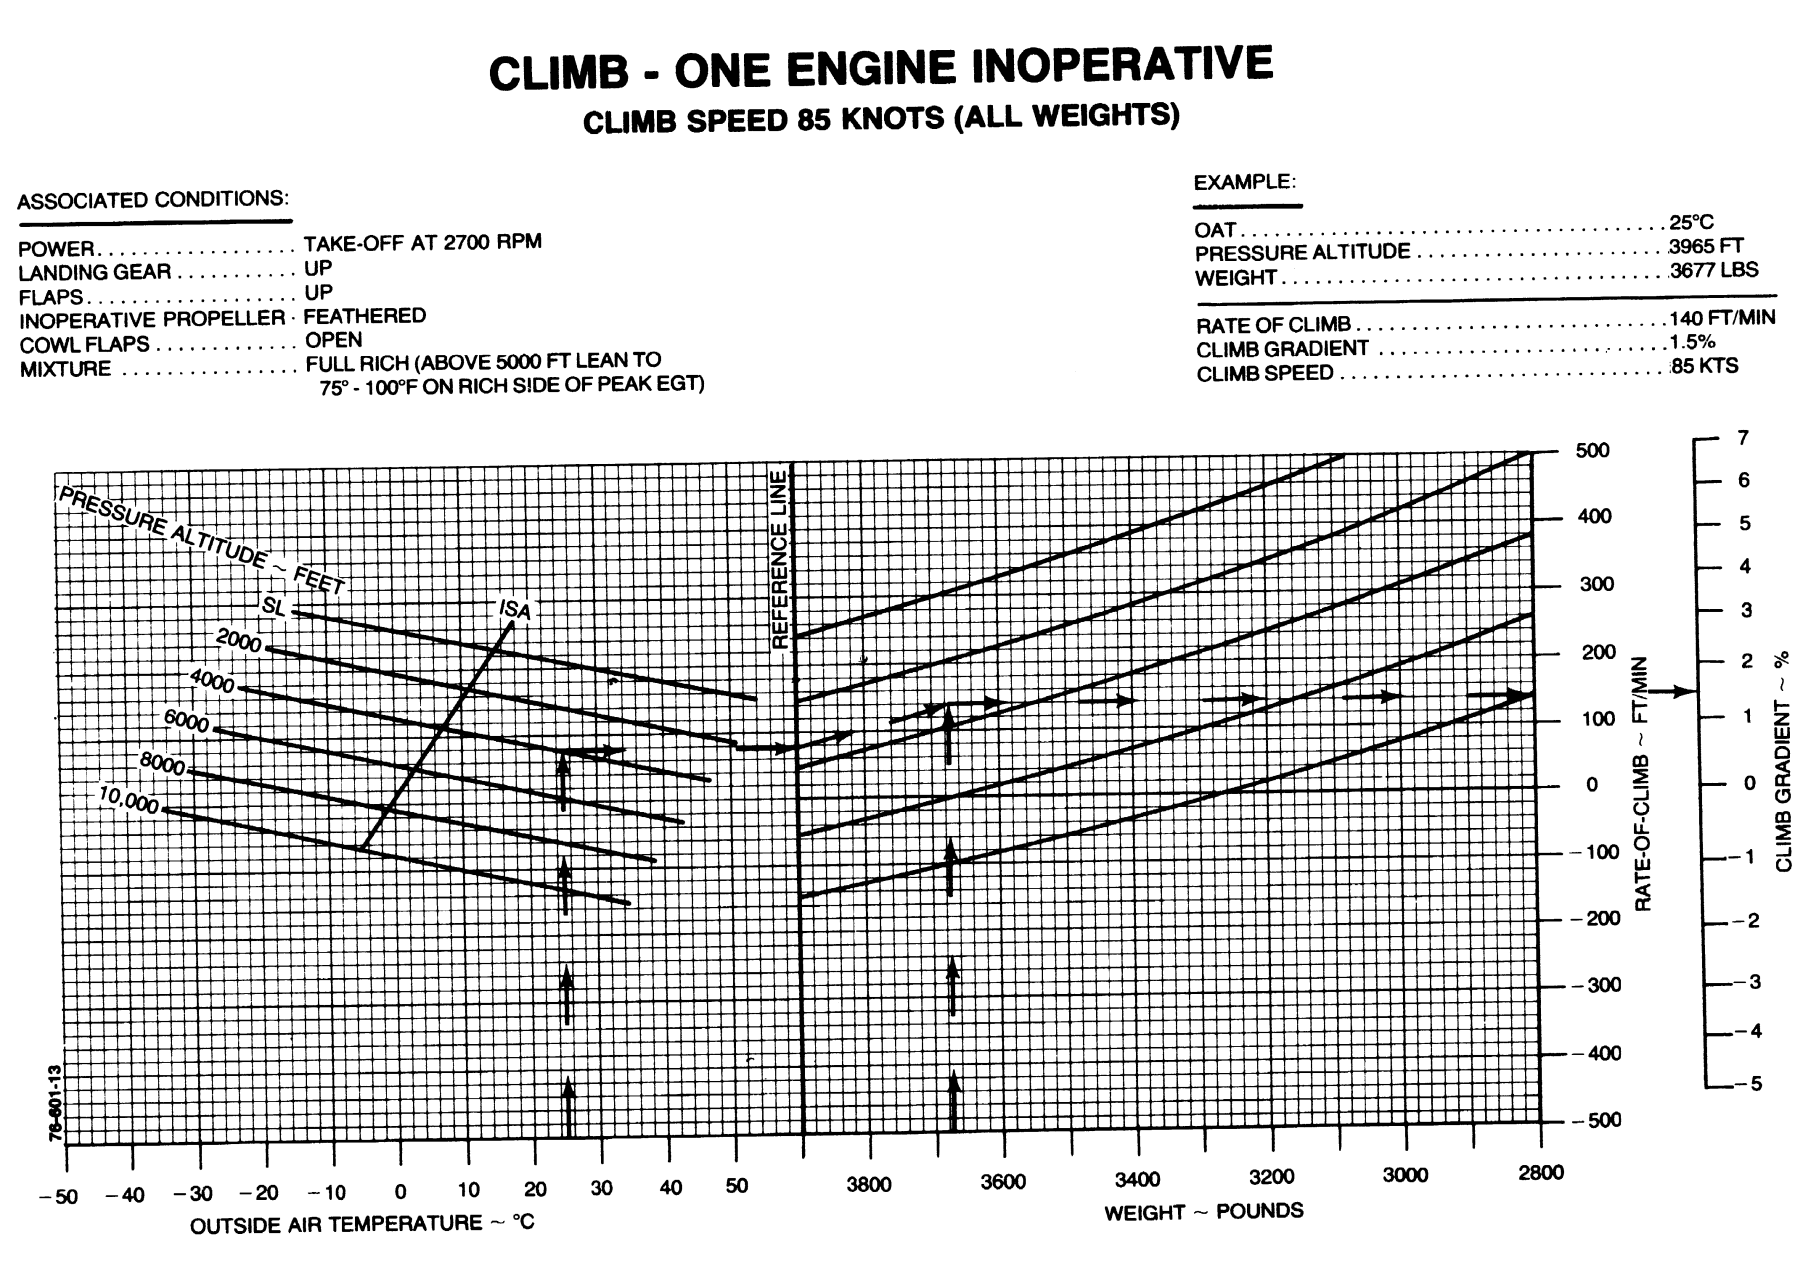
\includegraphics[width=0.9\linewidth]{duchess-1eo}
\end{center}
\end{figure}

\section{Time, Fuel, and Distance to Climb}

\begin{figure}[H]
\begin{center}
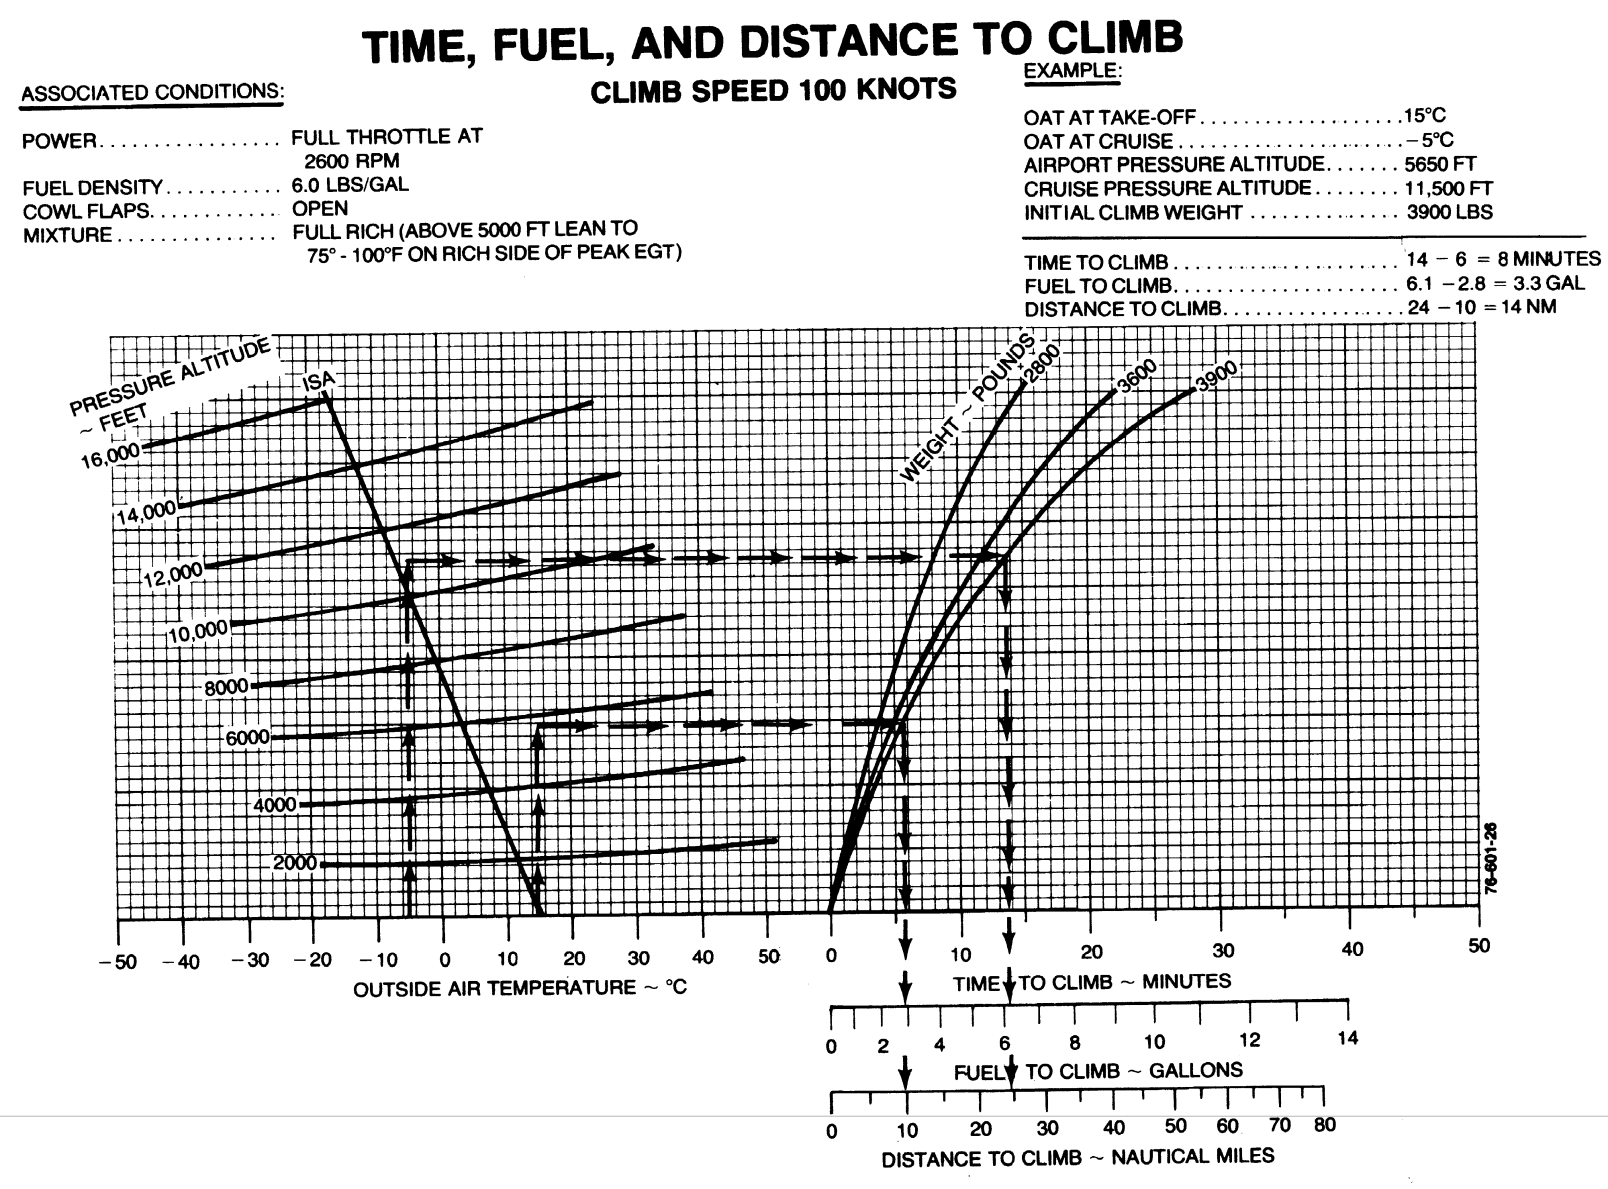
\includegraphics[width=1.0\linewidth]{duchess-tfd}
\end{center}
\end{figure}

\emph{Example:}

\begin{table}[H]
\begin{tabular}{l|l|l|l}
      & \multicolumn{1}{c|}{\begin{tabular}[c]{@{}c@{}}Min\\ T\end{tabular}} & \multicolumn{1}{c|}{\begin{tabular}[c]{@{}c@{}}Gal\\ F\end{tabular}} & \multicolumn{1}{c}{\begin{tabular}[c]{@{}c@{}}NM\\ D\end{tabular}} \\ \hline
4500  & 3.5                                                                  & 1.9                                                                  & 6                                                                   \\ \hline
GTU   & 0.2                                                                  & 0.1                                                                  & 1                                                                   \\ \hline
Climb & 3                                                                    & 1.8                                                                  & 5                                                                  
\end{tabular}
\end{table}

\newpage

\section{Single-Engine Service Ceiling}

\begin{figure}[H]
\begin{center}
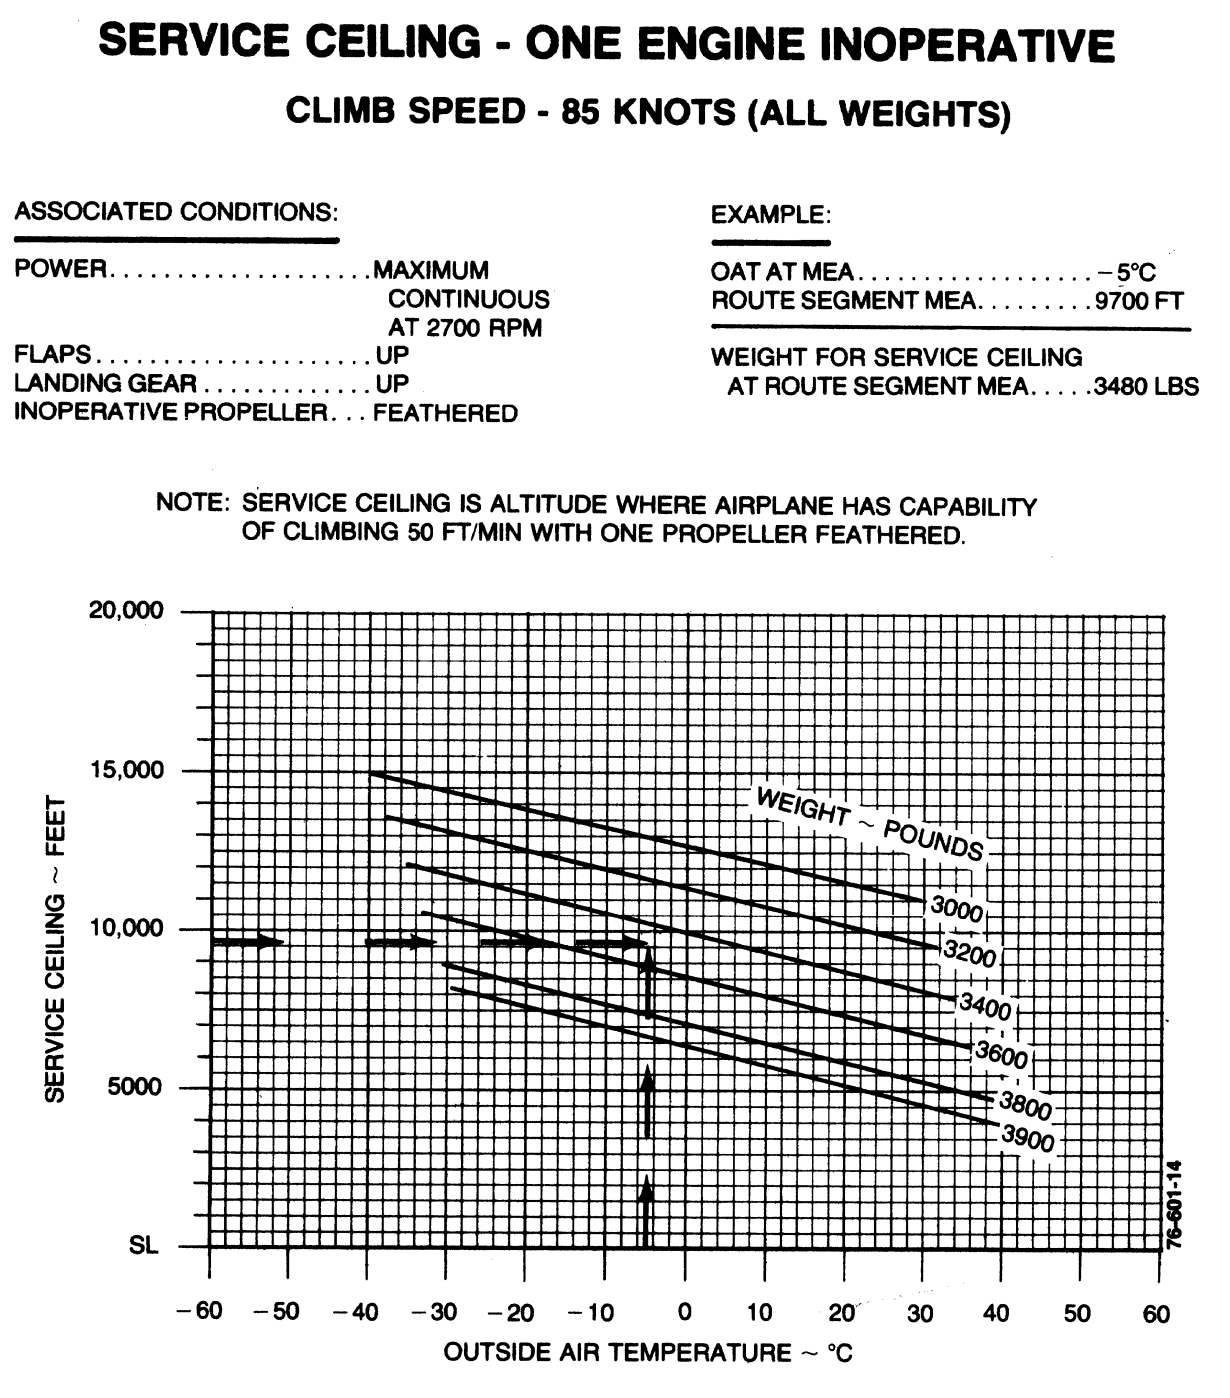
\includegraphics[width=1.0\linewidth]{duchess-secc}
\end{center}
\end{figure}

\newpage

\section{Cruise Performance, 24” Hg}

\begin{figure}[H]
\begin{center}
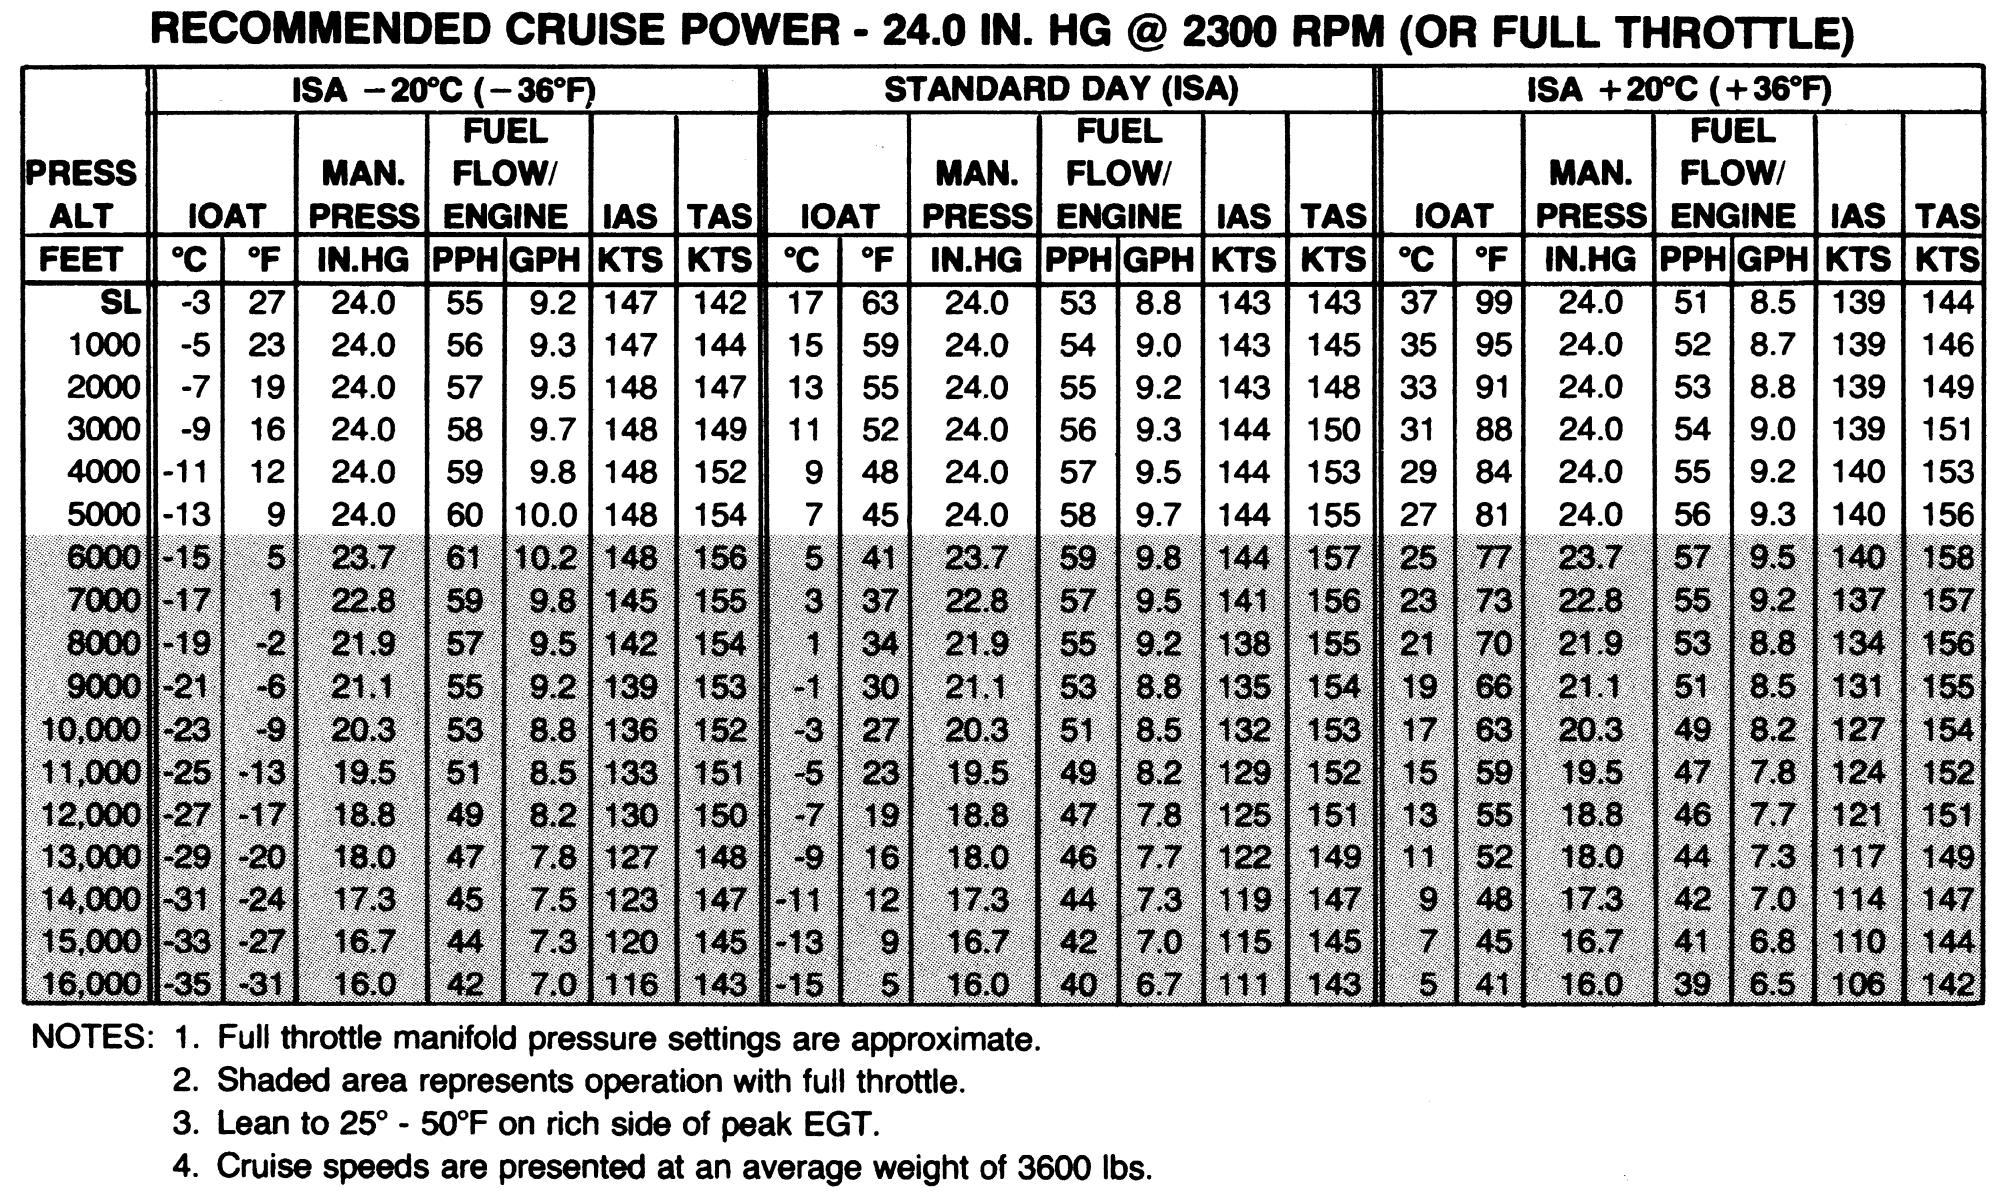
\includegraphics[width=0.9\linewidth]{duchess-24in}
\end{center}
\end{figure}

\section{Cruise Performance, 20” Hg}

\begin{figure}[H]
\begin{center}
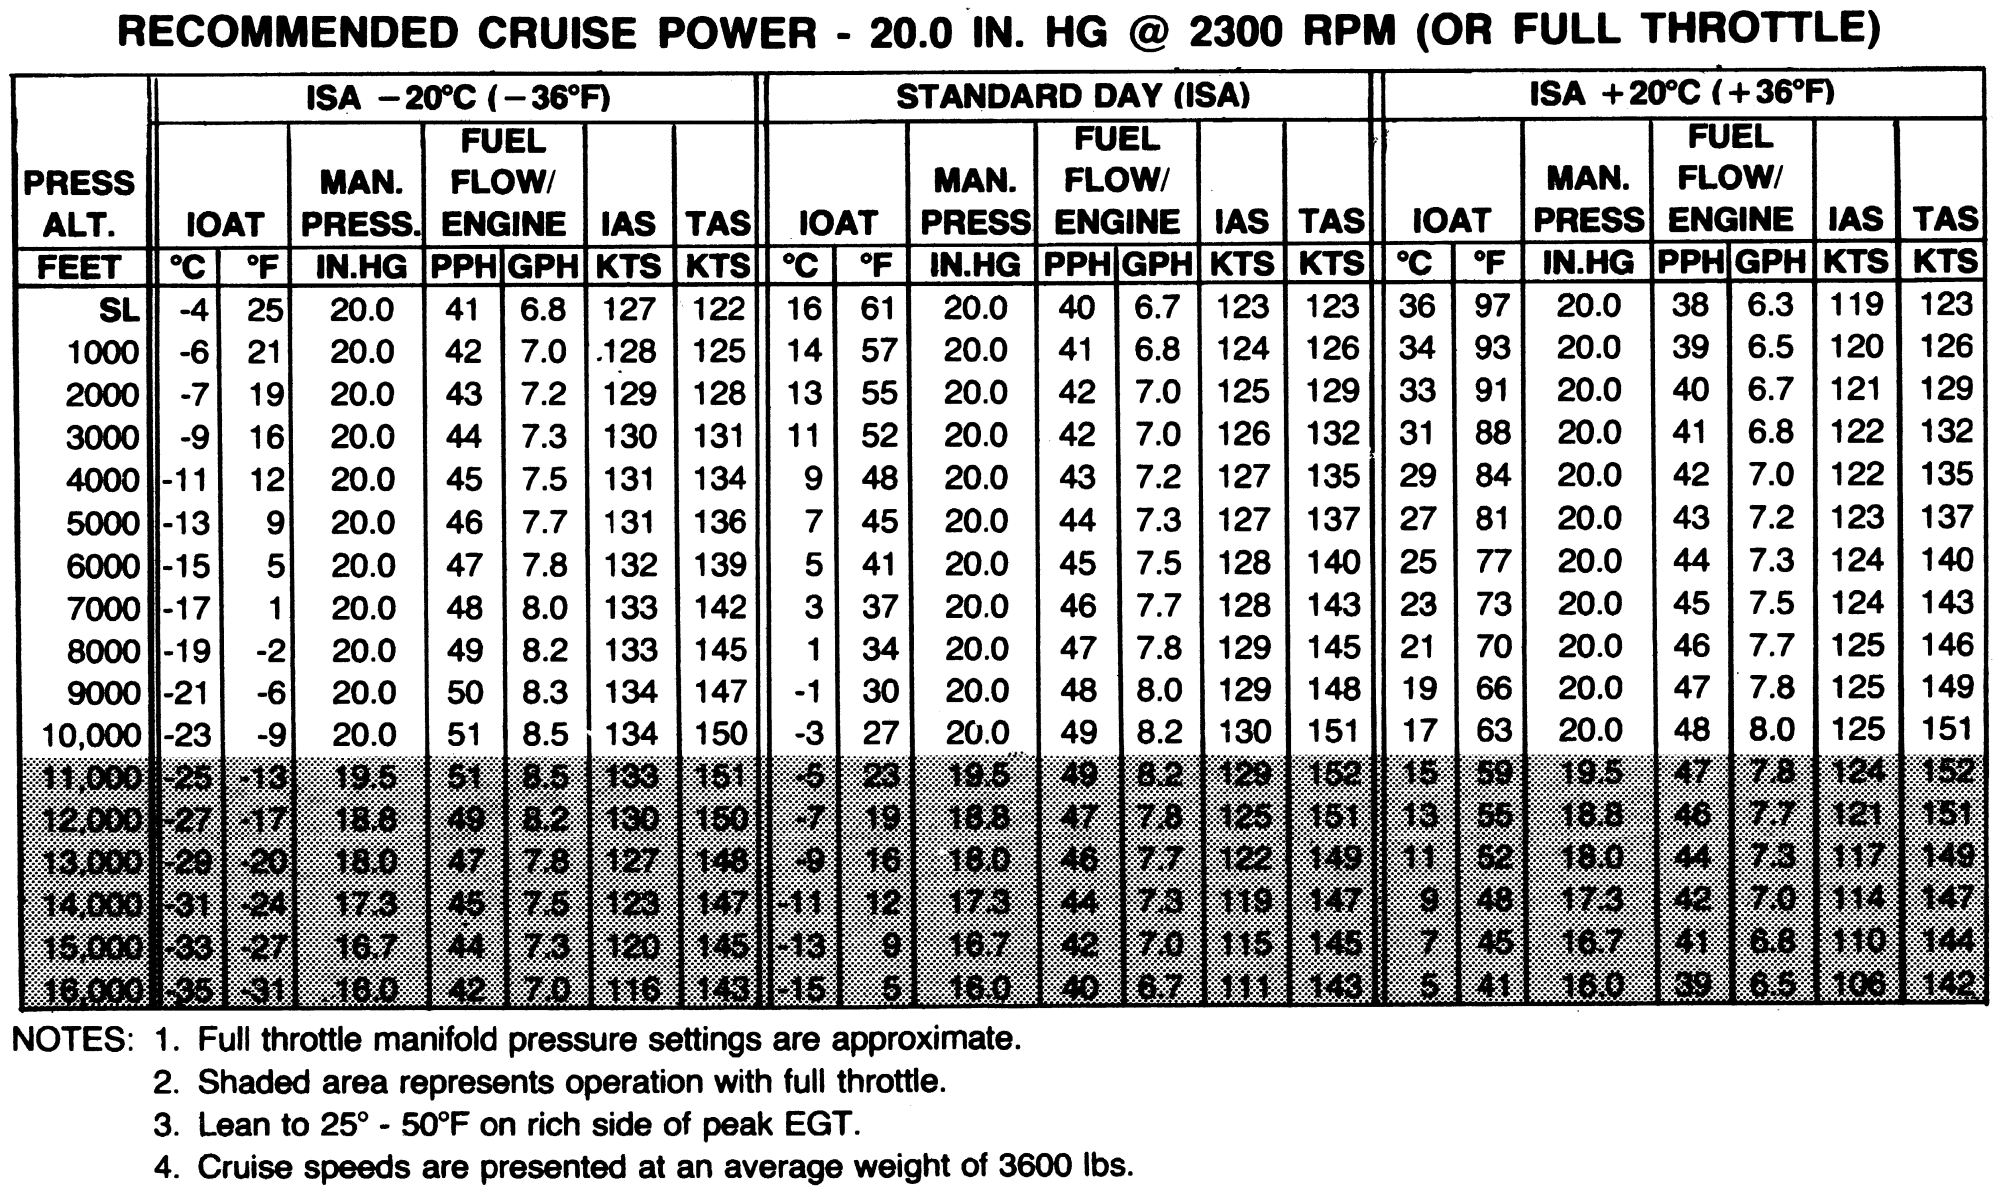
\includegraphics[width=0.9\linewidth]{duchess-20in}
\end{center}
\end{figure}

\newpage

\section{Landing Distance}

\begin{figure}[H]
\begin{center}
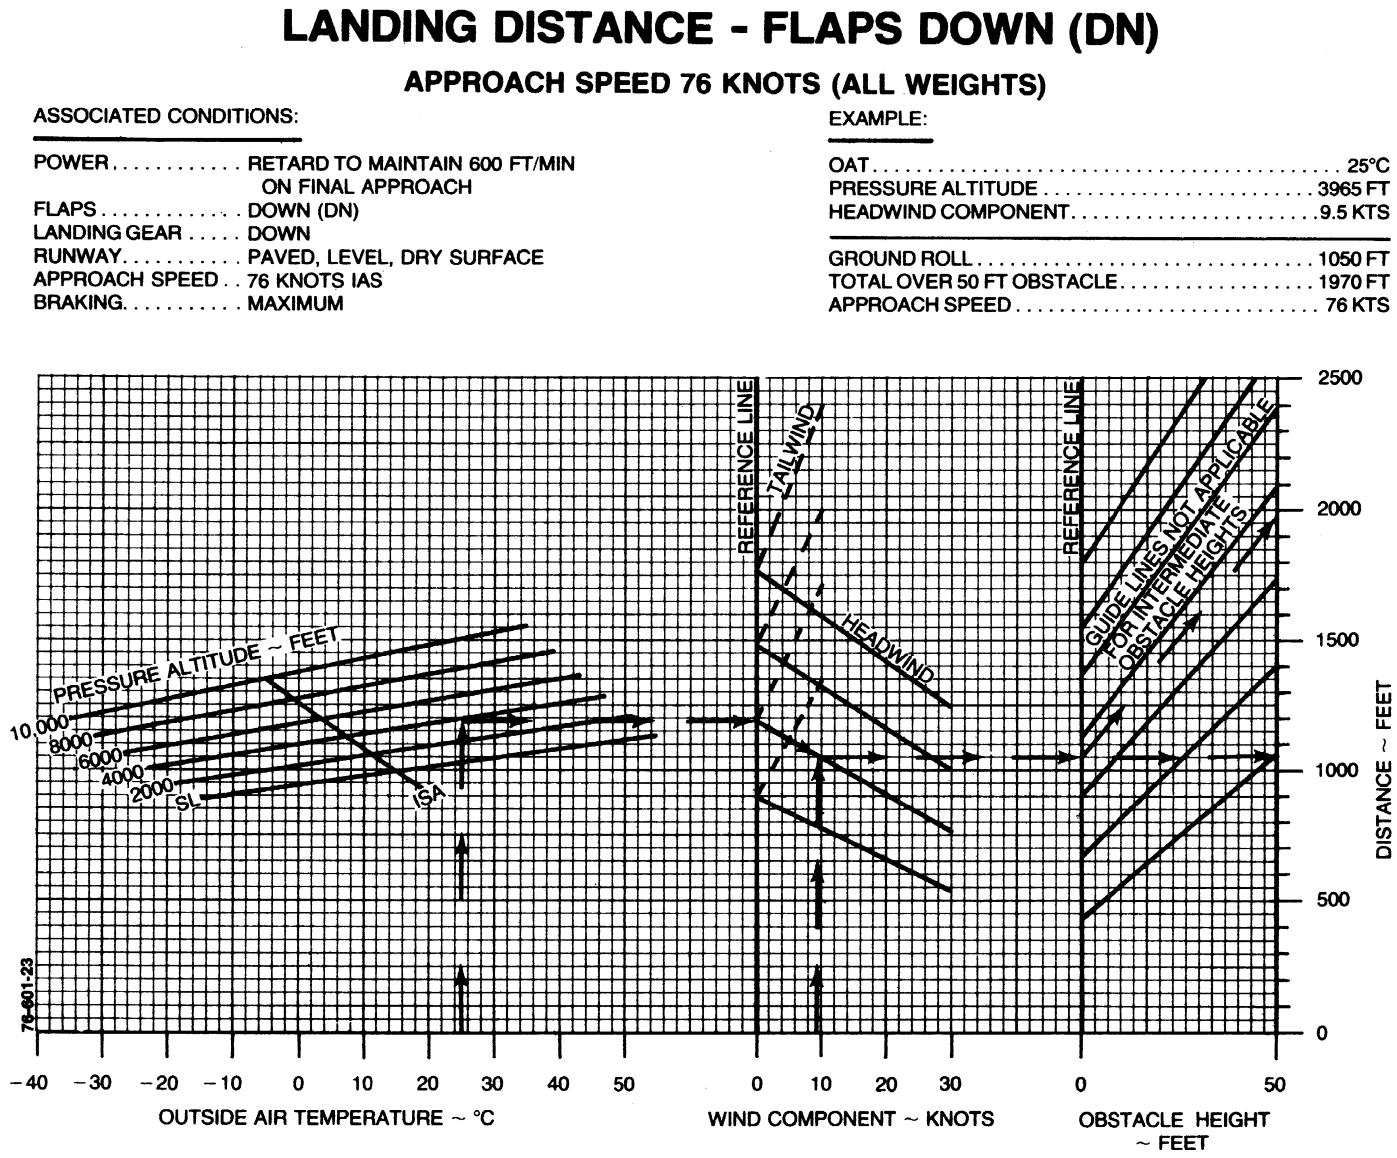
\includegraphics[width=1.0\linewidth]{duchess-ldg}
\end{center}
\end{figure}

